\documentclass[a4paper,11pt]{article}

%\usepackage[utf8]{inputenc}
\usepackage[T1]{fontenc}
\usepackage{fullpage}
\usepackage{parskip}
\usepackage{amsmath}
\usepackage{amssymb}
\usepackage{listings}
\usepackage{color}
\usepackage{xcolor}
\usepackage{float}
\usepackage{graphicx}
\usepackage[bookmarks=true,pdfborder={0 0 0}]{hyperref}
\usepackage{subcaption}

\providecommand{\e}[1]{\ensuremath{10^{#1}}}

\lstset{
  language=matlab,                	% choose the language of the code
  basicstyle=\footnotesize,       % the size of the fonts that are used for the code
  numbers= left,                 	% where to put the line-numbers
  numberstyle=\footnotesize,      % the size of the fonts that are used for the line-numbers
  stepnumber=1,                   % the step between two line-numbers. If it is 1 each line will be numbered
  numbersep=5pt,                  % how far the line-numbers are from the code
  backgroundcolor=\color{white},  % choose the background color. You must add \usepackage{color}
  showspaces=false,               % show spaces adding particular underscores
  showstringspaces=false,         % underline spaces within strings
  showtabs=false,                 % show tabs within strings adding particular underscores
  frame=single,           		% adds a frame around the code
  tabsize=2,          			% sets default tabsize to 2 spaces
  captionpos=t,          			% sets the caption-position to bottom (t=top, b=bottom)
  breaklines=true,        		% sets automatic line breaking
  breakatwhitespace=false,    	% sets if automatic breaks should only happen at whitespace
  escapeinside={\%*}{*)}          % if you want to add a comment within your code
}

\title{MSc Computer Vision 2014-2015\\Advanced Image Analysis\\Wavelet Decomposition and Filter Bank}
\author{Marwan \textsc{Osman}\\ marwan.aosman@gmail.com\\ MSCV 5}
\date{}

\begin{document}
\maketitle

This report will show the results of implementing a simple wavelet transform using the Daubechies D4 filter, and its application to image denoising.

\section*{Implementation}
The required wavelet transform is implemented in the function \texttt{fwt\_2d\_marwan.m}. This function computes the \texttt{j-level} wavelet transform of an input $NxN$ image. The function has the following inputs:
\begin{itemize}
  \item \textbf{mode}: Indicates whether to compute the forward or inverse wavelet transform. \texttt{0} indicates forward, \texttt{1} indicates inverse.
  \item \textbf{input}: This is the input $NxN$ image to be transformed. N is assumed to be a power of 2.
  \item \textbf{nlevel}: The required number of levels to compute for the wavelet transform.
  \item \textbf{h}: The Analysis low pass filter used for the transform.
\end{itemize}

And the \textbf{output} of the function is the wavelet transform coefficients, if the transform was forward, or the reconstructed image, if the transform was inverse.

The function is implemented as a recursive function, since for each level we need to compute the transform for half of the coefficients for next level. First, we construct the high pass filter from given low pass filter. Depending on the transform mode, we begin computing the transform.

Forward wavelet transform is applied on the input image on each row first. Then it is applied again on the temporary output of the previous operation but this time on each column. If we still have more levels to compute, the function is recursively called again and given the first quadrant of coefficients which is relevant to the transform.

Inverse wavelet transform is similar to the forward one, except that the inverse transform is called recursively on the first quadrant of coefficients, then applied on each column then on each row. It follows the inverse steps of the forward implementation.

\section*{Results}
For analysing the application of wavelet transform on denoising images, we start by adding Gaussian white noise on the test image. Then we compute the transform coefficients.

There are two methods of thresholding noise: Soft Threshold and Hard Threshold. The difference between the results of the two methods is shown in Fig.\ref{comparison}. We can notice that the Soft Thresholding adds blurring to the image and looses edge information much more than Hard Thresholding. This is expected as Soft Thresholding is not preserving the original wavelet coefficients values, but rather keeping the difference between the coefficients and the thresholding parameter.
\begin{figure}[ht!]
  \centering
  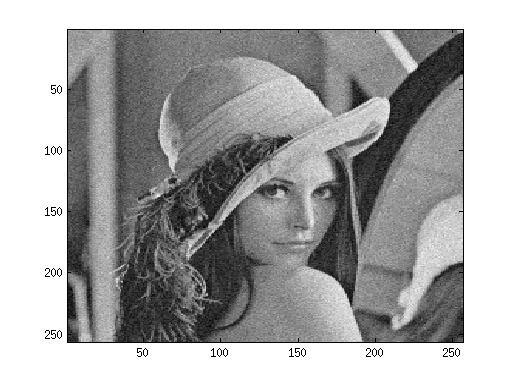
\includegraphics[width=80mm]{noisylena.png}
  \caption{Testing Noisy Image Input}
  \label{noisy}
\end{figure}

\begin{figure}[ht!]
  \centering
  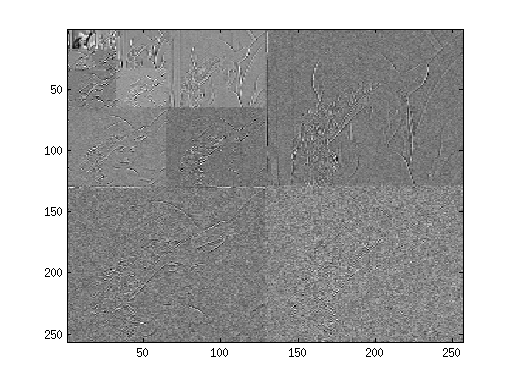
\includegraphics[width=100mm]{transform.png}
  \caption{Wavelet Transform for Noisy Lena Image}
  \label{transform}
\end{figure}

\begin{figure}[ht!]
  \centering
  \begin{subfigure}{.50\textwidth}
    \centering
    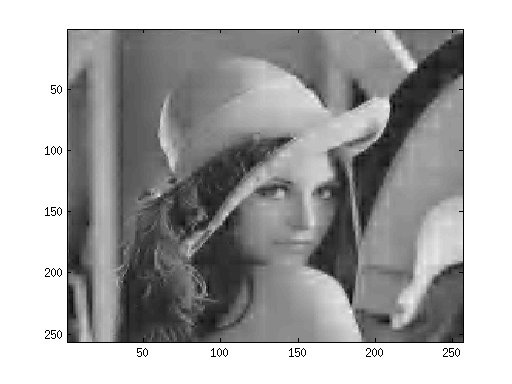
\includegraphics[width=80mm]{thresholding_soft.png}
  \end{subfigure}%
  \begin{subfigure}{.50\textwidth}
    \centering
    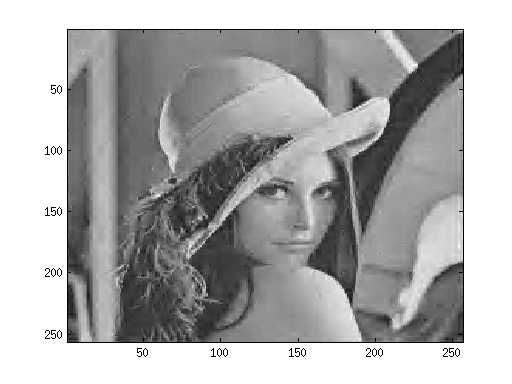
\includegraphics[width=80mm]{thresholding_hard.png}
  \end{subfigure}%
  \caption{The difference between soft and hard thresholding the coefficients of the wavelet transform.}
  \label{comparison}
\end{figure}

\end{document}
